% section
\section{Machine Learning Theory}
 % subsection
 \subsection{Image Prediction}
  \begin{frame}
   \frametitle{Image Prediction}
   
   \begin{itemize}
    \item<1-> Field inside machine learning / computer vision
    \item<2-> Predict future image/s, given sequence of images
    \item<3-> $X$ the image sequence of length $n$
    \item<4-> with $X = (x_0, \ldots, x_{n-1})$
    \item<5-> Two possible use-cases
    \begin{itemize}
     \item<6-> One-frame prediction
     \begin{itemize}
      \item<7-> Predicting $x_n$
     \end{itemize}
     \item<8-> Multi-frame prediction
     \begin{itemize}
      \item<9-> Predict $t > 1$ frames into the future $(x_n, \ldots, x_{n+t-1})$
      \item<10-> Often it is one-frame prediction in a feedback loop
      \item<11-> Propagate the error $\rightarrow$ Greater error in later images
     \end{itemize}
    \end{itemize}
   \end{itemize}
   
  \end{frame}
 
 % subsection
 \subsection{Autoencoder}
  \begin{frame}
   \frametitle{Autoencoder}
   
   \begin{itemize}
    \item<1-> Two networks chained together
    \begin{itemize}
     \item<2-> Encoder
      \begin{itemize}
       \item<3-> Input is $x$
       \item<4-> Output is $h$\footnote{$h$ is the so named \textbf{code}. Output layer is named \textbf{bottleneck layer}.}
       \item<5-> $E(x) = h$
      \end{itemize}
     \item<6-> Decoder
     \begin{itemize}
      \item<7-> Input is $h$
      \item<8-> Output is $x\prime$
      \item<9-> $D(h) = x\prime$
     \end{itemize}
    \end{itemize}
    \item<10-> Used for reconstruction $x \approx x\prime$
    \item<11-> Important is to prevent the network to simply copy $x$ to $x\prime$ (Interpolation)
    \item<12-> Simplest architecture is the undercomplete autoencoder
    \begin{itemize}
     \item<13-> Code smaller then input
     \item<14-> Network needs to distinguish between useful and obsolete
    \end{itemize}
   \end{itemize}
  
  \end{frame}
  \begin{frame}
   \frametitle{Autoencoder}
   
   \begin{figure}[H]
    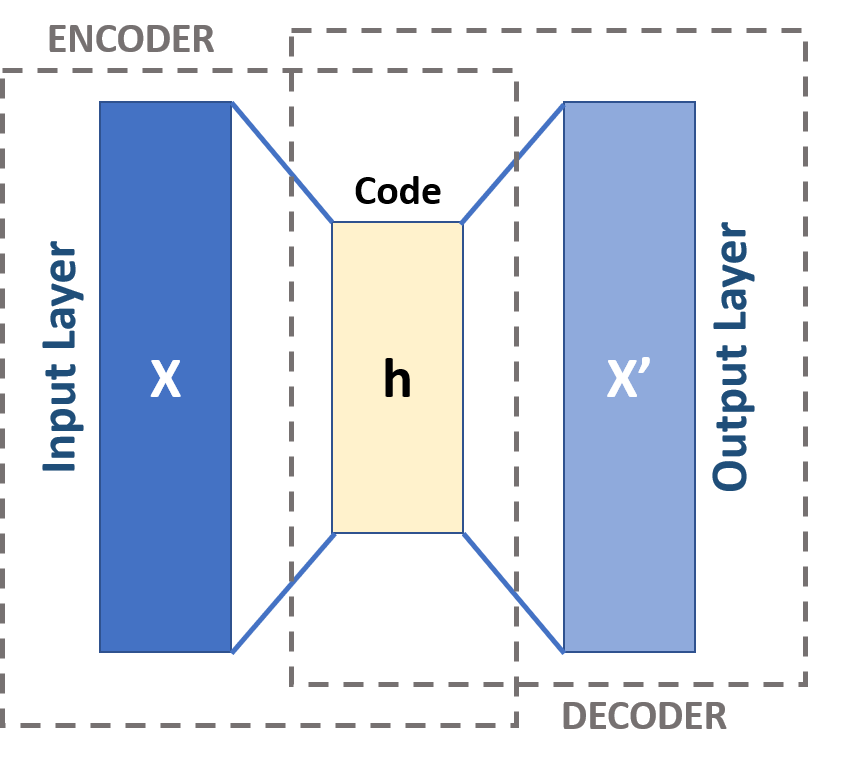
\includegraphics[width=0.38\textwidth]{../Images/autoencoder_schema.png}
    \centering
    \caption{Autoencoder schema \cite{wiki2019}}
    \label{fig:lstm_architecture}
   \end{figure}
   
  \end{frame}
 
 % subsection
 \subsection{CNN}
  \begin{frame}
   \frametitle{CNN}
   
   \begin{itemize}
    \item<1-> Convolutional Neural Network
    \item<2-> Consists of three stages
    \begin{enumerate}
     \item<3-> Convolutional layer
     \item<4-> Non-linearity (ReLU, sigmoid, $\ldots$)
     \item<5-> Pooling layer
    \end{enumerate}
   \end{itemize}
   \onslide<6->{
    \begin{figure}[H]
     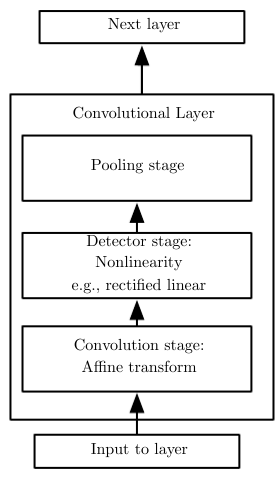
\includegraphics[width=0.2\textwidth]{../Images/convlayer.png}
     \centering
     \caption{Stages of a CNN \cite{Goodfellow2016}}
     \label{fig:cnn_stage}
    \end{figure}
   }

  \end{frame}
  \begin{frame}
   \frametitle{CNN (First stage)}
   
   \begin{itemize}
    \item<1-> Discrete convolutional operation
    \item<2-> $(I \ast K)(i,j) = \sum_m\sum_nI(m,n)K(i-m,j-n)$
   \end{itemize}
   \onslide<3->{
   \begin{figure}[H]
    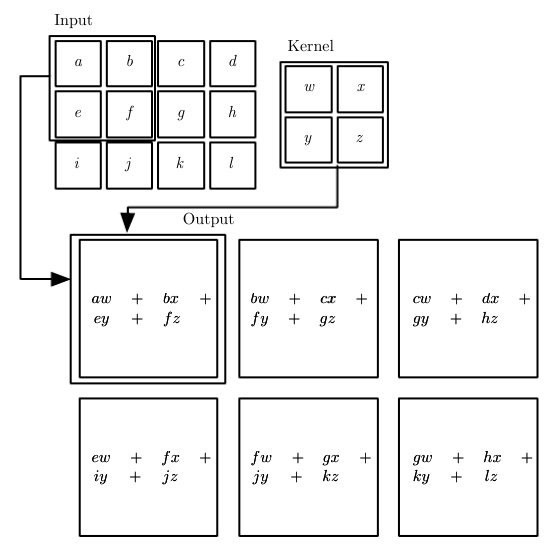
\includegraphics[width=0.45\textwidth]{../Images/kernel.png}
    \centering
    \caption{Two dimensional convolutional operation \cite{Goodfellow2016}}
    \label{fig:kernel}
   \end{figure}
   }
   
  \end{frame}
  \begin{frame}
   \frametitle{CNN (Second stage)}
   
   \begin{itemize}
    \item<1-> Non-linearity layer
    \item<2-> ReLU: $R(x) = max(0,x)$
    \item<3-> Sigmoid: $\sigma(x) = \frac{1}{1+e^{-x}}$
   \end{itemize}
   
  \end{frame}
  \begin{frame}
   \frametitle{CNN (Third stage)}
   
   \begin{itemize}
    \item<1-> Pooling layer
    \item<2-> Aggregate output / Making output invariant to input
    \item<3-> E.g. Max-Pooling
   \end{itemize}
   \onslide<4->{
    \begin{figure}[H]
     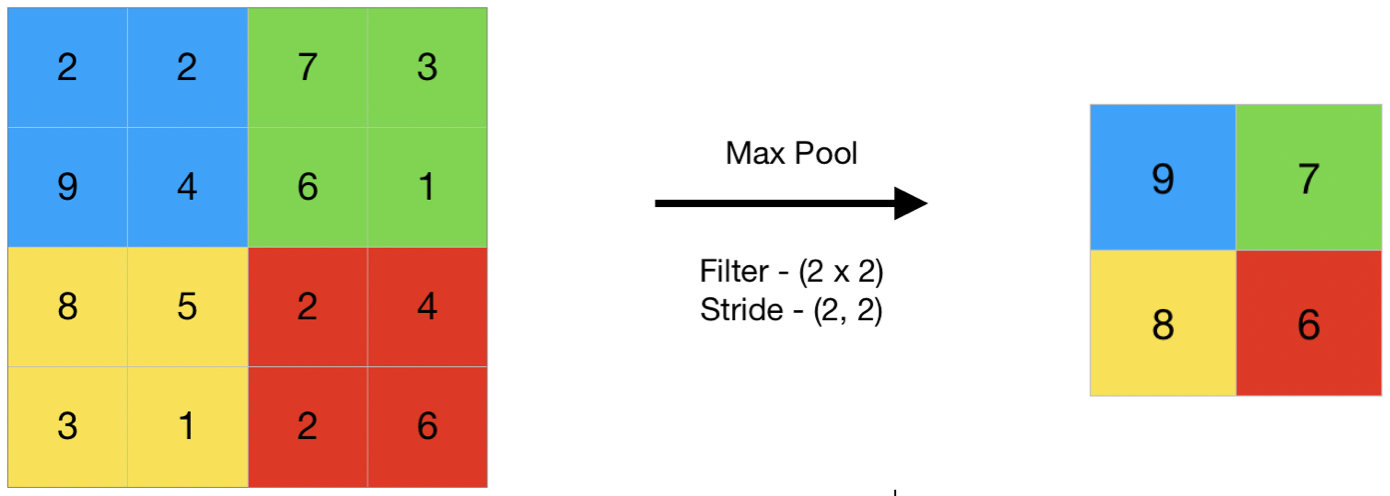
\includegraphics[width=0.6\textwidth]{../Images/max_pooling.png}
     \centering
     \caption{Max-Pooling (Filter $:=$ Kernel)\cite{savyakhosla2019}}
     \label{fig:max_pooling}
    \end{figure}
   }    
  
  \end{frame}
 
 % subsection
 \subsection{RNN}
  \begin{frame}
   \frametitle{RNN}
   
   \begin{itemize}
    \item<1-> Recurrent Neural Network
    \item<2-> Handling sequential data
    \item<3-> $X = (x_0, \ldots, x_{t-1})$, $|X| = t$
    \item<4-> Used for e.g. time-series analysis, image-/video-prediction
    \item<5-> Gets output of last iteration as \glqq additional\grqq input
    \item<6-> $\hat{y}^t = f_{\theta}(\hat{y}^{t-1};x^t) = f_{\theta}(f_{\theta}(\hat{y}^{t-2};x^{t-1});x^t) = \ldots$
    \item<7-> Requires $\hat{y}^0$ to be initialized (Often done with zero)
    \item<8-> Typically trained using BPTT
   \end{itemize}
   
  \end{frame}
  \begin{frame}
   \onslide<1->{
    \begin{figure}[H]
     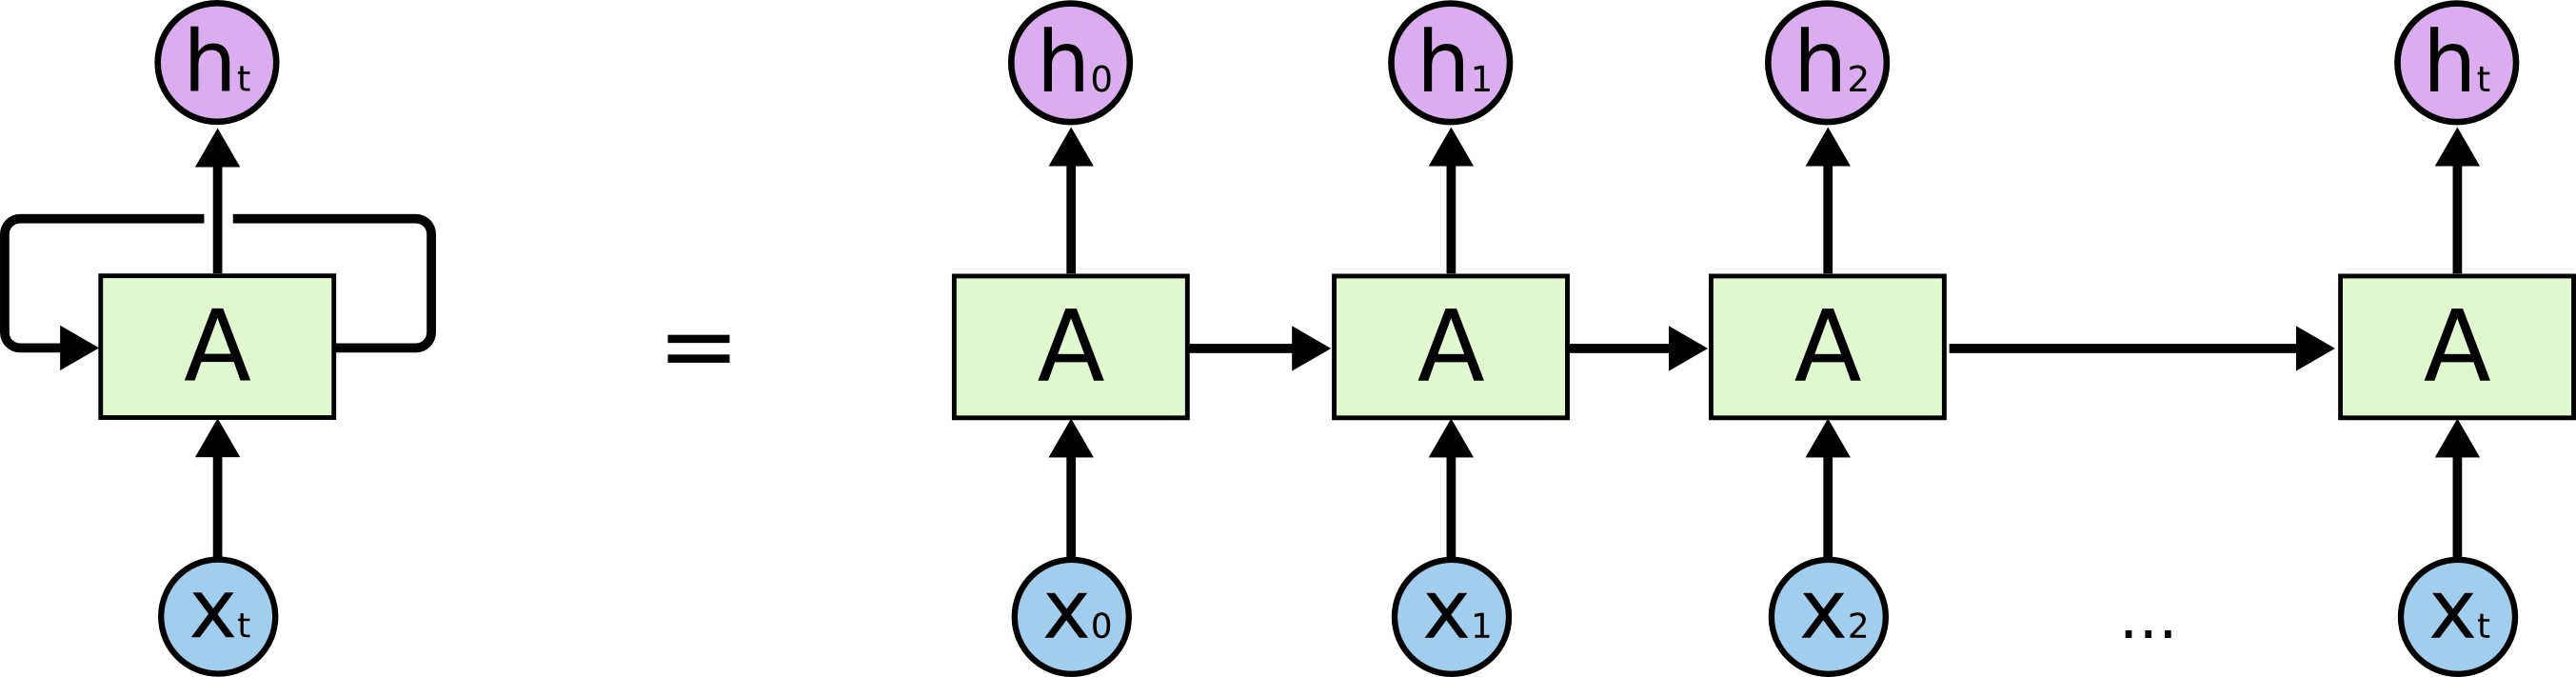
\includegraphics[width=0.8\textwidth]{../Images/rnn.png}
     \centering
     \caption{RNN schema. \textbf{Left:} Folded graph, \textbf{Right:} Unfolded graph \cite{Olah2015}}
     \label{fig:lstm_architecture}
    \end{figure}
   }
  \end{frame}
 
 % subsection
 \subsection{LSTM}
  \begin{frame}
   \frametitle{LSTM}
   
   \begin{itemize}
    \item<1-> Long Short-term Memory
    \item<2-> Invented by Hochreiter and Schmidhuber \cite{Hochreiter1997}
    \item<3-> Avoids critical problem of standard RNN: Saving long-term dependencies
   \end{itemize}
   \onslide<4->{
    \begin{equation}
     i_t = \sigma(w_{x_i}x_t + w_{h_i}h_{t-1} + b_i)
    \end{equation}
   }
   \onslide<5->{
    \begin{equation}
     f_t = \sigma(w_{x_f}x_t + w_{h_f}h_{t-1} + b_f)
    \end{equation}
   }
   \onslide<6->{
    \begin{equation}
     c_t = f_tc_{t-1} + i_ttanh(w_{x_c}x_t + w_{h_c}h_{t-1} + b_c)
    \end{equation}
   }
   \onslide<7->{
    \begin{equation}
     o_t = \sigma(w_{x_o}x_t + w_{h_o}h_{t-1} + b_o)
    \end{equation}
   }
   \onslide<8->{
    \begin{equation}
     h_t = o_ttanh(c_t)
    \end{equation}
   }
   
  \end{frame}
  \begin{frame}
   \frametitle{LSTM}
   
   \onslide<1->{
    \begin{figure}[H]
     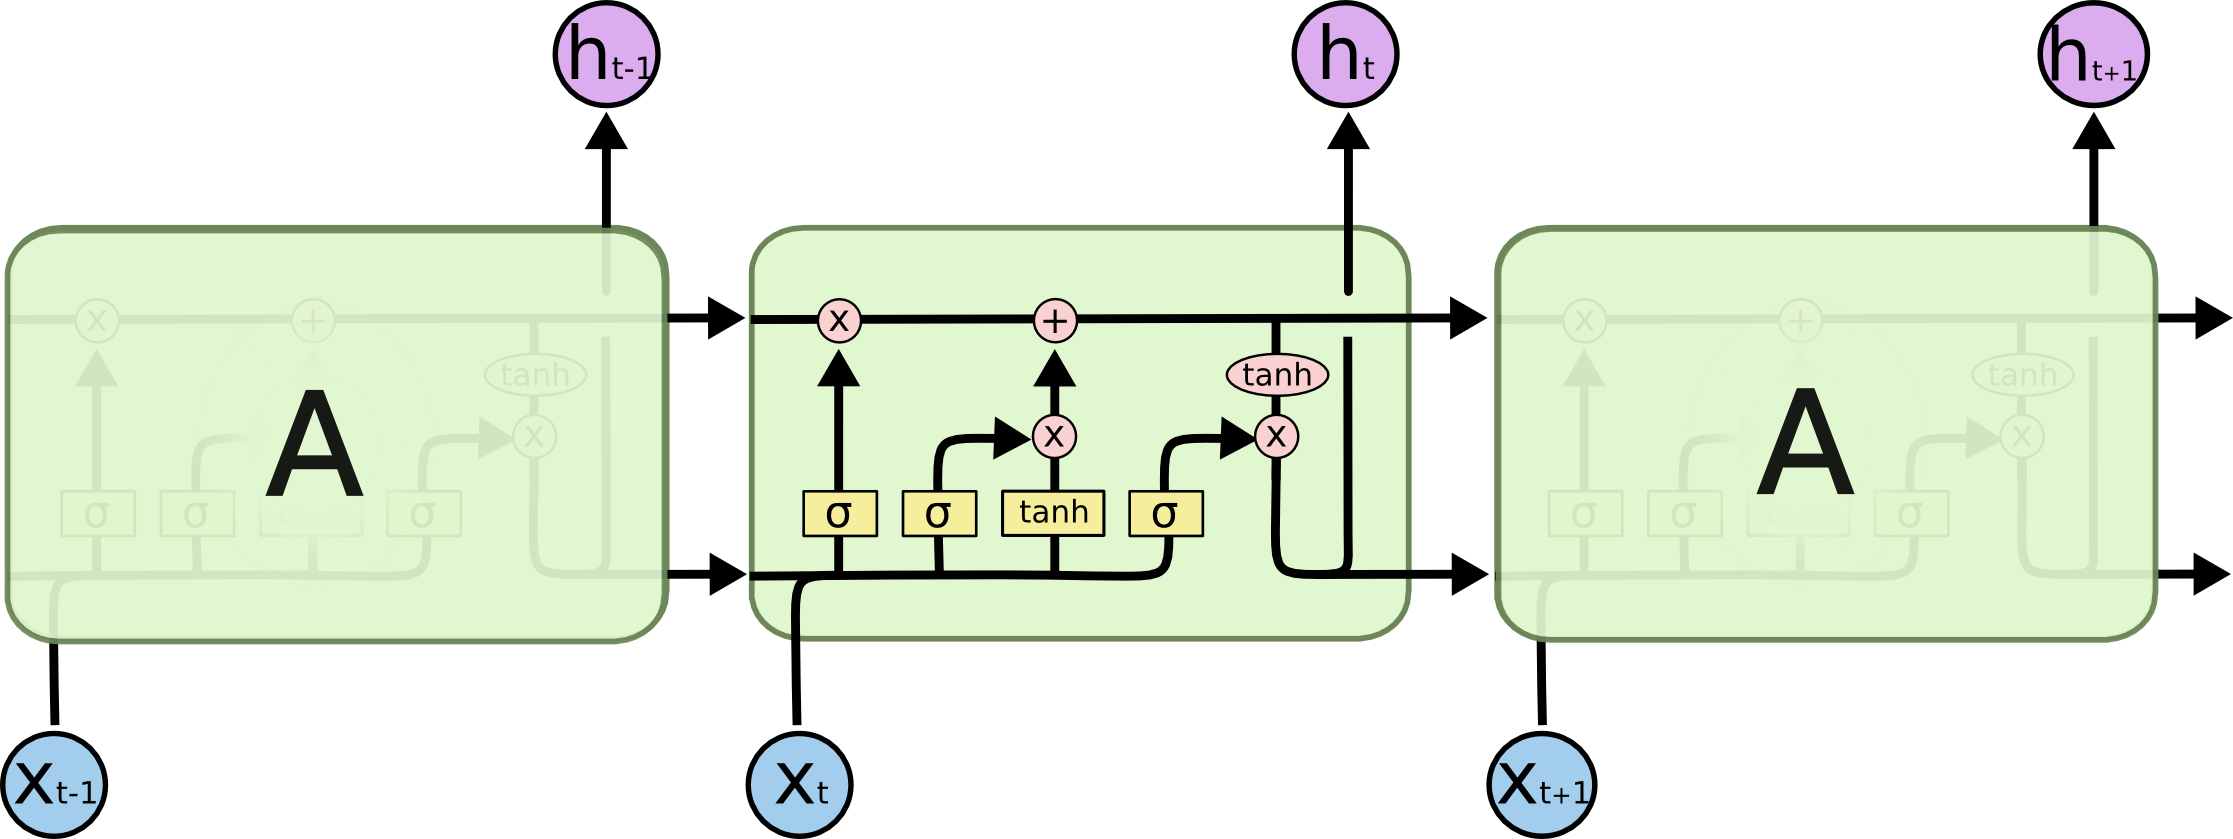
\includegraphics[width=0.7\textwidth]{../Images/lstm_chain.png}
     \centering
     \caption{LSTM Architecture \cite{Olah2015}}
     \label{fig:lstm_architecture}
    \end{figure}
   }
   \begin{itemize}
    \item<2-> Top horizontal line: Cell-state
   \end{itemize}
  
  \end{frame}
 
 % subsection
 \subsection{ConvLSTM}
  \begin{frame}
   \frametitle{ConvLSTM}
   
   \begin{itemize}
    \item<1-> Invented by Shi et al. \cite{Shi2015}
    \item<2-> LSTM with peephole using convlayer
   \end{itemize}
   \onslide<3->{
    \begin{equation}
     i_t = \sigma(x_t \ast w_{x_i} + h_{t-1} \ast w_{h_i} + w_{i_b})
    \end{equation}
   }
   \onslide<4->{
    \begin{equation}
     f_t = \sigma(x_t \ast w_{x_f} + h_{t-1} \ast w_{h_f} + w_{f_b})
    \end{equation}
   }
   \onslide<5->{
    \begin{equation}
     \tilde{c}_t = tanh(x_t \ast w_{x_{\tilde{c}}} + h_{t-1} \ast w_{h_{\tilde{c}}} + w_{\tilde{c}_b})
    \end{equation}
   }
   \onslide<6->{
    \begin{equation}
     c_t = \tilde{c}_t \odot i_t + c_{t-1} \odot f_t
    \end{equation}
   }
   \onslide<7->{
    \begin{equation}
     o_t = \sigma(x_t \ast w_{x_o} + h_{t-1} \ast w_{h_o} + w_{o_b})
    \end{equation}
   }
   \onslide<8->{
    \begin{equation}
     h_t = o_t \odot tanh(c_t)
    \end{equation}
   }
   
  \end{frame}
 
 % subsection
 \subsection{Backpropagation}
  \begin{frame}
   \frametitle{Backpropagation}
   
   \begin{itemize}
    \item<1-> Backpropagation was invented by Rumelhart et al. \cite{Rumelhart1986} in 1986.
    \item<2-> Most used algorithm for training neural nets.
    \item<3-> Simple example on Perceptron \cite{Rosenblatt1957}.
   \end{itemize}      
   \onslide<4->{
   \begin{center}
    \begin{tikzpicture}[roundnode/.style={circle, draw=green!60, fill=green!5, very thick, minimum size=7mm},
  					 roundnodesmall/.style={circle, draw=green!60, fill=green!5, thick, minimum size=1mm}]
    % Node
    \node[roundnode] (circle) {$\sum | \sigma$};
    \node[roundnodesmall] (x1) [above left=of circle] {$x_1$};
    \node[roundnodesmall] (x2) [below left=of circle] {$x_2$};
    \node[roundnodesmall] (y) [right=of circle] {$\hat{y}$};
    % Lines
    \draw[->, bend left=45] (x1.east) -- (circle) node[above left=1.2cm] {$w_1$};
    \draw[->] (x2.east) -- (circle) node[below left=1.2cm] {$w_2$};
    \draw[->] (circle) -- (y);
   \end{tikzpicture}
  \end{center}
  }
   
  \end{frame}
  \begin{frame}
   \frametitle{Backpropagation Forward Pass}
   
   \onslide<1->\textbf{Forward Pass:}
   \begin{itemize}
    \item<2->{
     \begin{equation}
      \hat{y} = \sigma(\sum_{i=1}^{2}x_iw_i)
     \end{equation}         
    }
    \item<3-> $\sigma$ is the sigmoid function
    \item<4->{
     \begin{equation}
      \sigma(x) = \frac{1}{1+e^{-x}}
     \end{equation}
    }
    \item<5-> Computing the error with e.g. \textbf{MSE}
    \item<6->{
    \begin{equation}
     L(y,\hat{y}) = \frac{1}{N}||y-\hat{y}||_2^2 = \frac{1}{N}\sum_{i=1}^N(y_i-\hat{y}_i)^2
    \end{equation}        
    }
   \end{itemize}    
  
  \end{frame}
  \begin{frame}
   \frametitle{Backpropagation Backward Pass}
   
   \onslide<1->\textbf{Backward Pass:}
   
   \begin{itemize}
    \item<2->{
    \begin{equation}
     \frac{\partial L}{\partial \hat{y}} = \frac{2}{N}\sum_{i=1}^N(y_i-\hat{y}_i)
    \end{equation}        
    }
    \item<3->{
    \begin{equation}
     \frac{\partial \sigma(x)}{\partial x} = \sigma(x)(1-\sigma(x))
    \end{equation}        
    }
    \item<4->{
    \begin{equation}
     \frac{\partial L}{\partial \sum_{i=1}^{2}x_iw_i} = \frac{\partial L}{\partial \hat{y}} \cdot \frac{\partial \hat{y}}{\partial \sum_{i=1}^{2}x_iw_i} = 
     \frac{2}{N}\sum_{i=1}^{N}(y_i-\hat{y}_i) \cdot \sigma(\sum_{i=1}^{2}x_iw_i)(1-\sigma(\sum_{i=1}^{2}x_iw_i))
    \end{equation}        
    }
    \item<5->{
    \begin{equation}
     \frac{\partial L}{\partial w_1} = \ldots = \frac{2}{N}\sum_{i=1}^{N}(y_i-\hat{y}_i) \cdot \sigma(\sum_{i=1}^{2}x_iw_i)(1-\sigma(\sum_{i=1}^{2}x_iw_i)) \cdot 
     x_1
    \end{equation}        
    }
   \end{itemize}
  
  \end{frame}
  \begin{frame}
   \frametitle{Backpropagation Update}
   
   \onslide<1-> Update weights using Gradient Descent
   
   \begin{itemize}
    \item<2->{
    \begin{equation}
     w_1 = w_1^{old} - \lambda \cdot \frac{\partial L}{\partial w_1}
    \end{equation}        
    }
    \item<3-> $\lambda$ is the learning rate
    \item<4-> All steps are performed iterative, until convergence
    \item<5-> It would be also possible to use e.g. Newton instead of Gradient Descent
    \begin{itemize}
     \item<6-> Gradient Descent is used more, because of its simplicity
     \item<7-> and because of its parallelism properties \cite{Rumelhart1986}
    \end{itemize}
   \end{itemize}
  
  \end{frame}

 % subsection
 \subsection{BPTT}
  \begin{frame}
   \frametitle{BPTT}
   
   \begin{itemize}
    \item<1-> Backpropagation through time
    \item<2-> Invented by Paul Werbos \cite{Werbos1990}
    \item<3-> Unfolding graph during backpass and propagate through the steps
    \item<4-> Simple example on RNN found in Goodfellow \cite{Goodfellow2016}
   \end{itemize}
   
  \end{frame}
  \begin{frame}
   \frametitle{BPTT Forward Pass}
   
   \onslide<1-> \textbf{Forward Pass:}
   
   \begin{itemize}
    \item<2->{
    \begin{align}
     h_t = tanh(Wh_{t-1} + Ux_t+b_1) \\
     o_t = Vh_t + b_2 \\
     \hat{y}_t = \sigma(o_t)
    \end{align}        
    }
    \item<3-> $U,V,W$ weight matrices for input-to-hidden, hidden-to-output, hidden-to-hidden
    \item<4-> Computing the error with e.g. \textbf{MSE} for every iteration
    \item<5->{
    \begin{equation}
     L(y,\hat{y}) = \sum_t(L_t(y_t,\hat{y}_t))
    \end{equation}        
    }
   \end{itemize}     
  
  \end{frame}
  \begin{frame}
   \frametitle{BPTT Backward Pass}
   
   \onslide<1-> \textbf{Backward Pass:}
   
   \begin{itemize}
    \item<2->{
    \begin{equation}
     \frac{\partial L}{\partial V} = \sum_t\frac{\partial L_t}{\partial V}
    \end{equation}
    }
    \item<3->{
    \begin{equation}
     \frac{\partial L_t}{\partial \hat{y}_t} = \frac{2}{N}\sum_{i=1}^{N}(y_t^i-\hat{y}_t^i)
    \end{equation}
    }
    \item<4->{
    \begin{equation}
     \frac{\partial L_t}{\partial o_t} = \frac{\partial L_t}{\partial \hat{y}_t} \cdot \frac{\partial \hat{y}_t}{\partial o_t} = \frac{2}{N}\sum_{i=1}^{N}(y_t^i-
     \hat{y}_t^i) \cdot \sigma(o_t)(1- \sigma(o_t))
    \end{equation}
    }
    \item<5->{
    \begin{equation}
     \frac{\partial L_t}{\partial V} = \frac{\partial L_t}{\partial \hat{y}_t} \cdot \frac{\partial \hat{y}_t}{\partial o_t} \cdot \frac{\partial o_t}{\partial V} 
     = \frac{2}{N}\sum_{i=1}^{N}(y_t^i-\hat{y}_t^i) \cdot \sigma(o_t)(1-\sigma(o_t)) \cdot h_t
    \end{equation}
    }
    \item<6->{
    \begin{equation}
     \frac{\partial L}{\partial V} = \sum_t\frac{\partial L_t}{\partial V}
    \end{equation}
    }
   \end{itemize}     
  
  \end{frame}
  \begin{frame}
   \frametitle{BPTT Update}
   
   \onslide<1-> Update weights using Gradient Descent   
   
   \begin{itemize}
    \item<2->{
    \begin{equation}
     V = V^{old} - \lambda \cdot \frac{\partial L}{\partial V}
    \end{equation}
    }
   \end{itemize}
  
  \end{frame}
